\scanpage{19}
\[
(8)\quad\left\{\begin{aligned}
\varepsilon_0&=l_0^{\deleted{\unsure{-1}}}\sigma_0l_{\unsure{1|0}}^{\deleted{\unsure{-1}}}\\
\varepsilon_1&=l_{\unsure{1|\infty}}^{\deleted{\unsure{-1}}}\sigma_{\unsure{1|\infty}}l_{\unsure{\infty|0}}^{\deleted{\unsure{-1}}}\\
\varepsilon_\infty&=l_\infty\sigma_\infty l_{\unsure{0|\infty}}^{\deleted{\unsure{-1}}}
\end{aligned}\right.
\]
\margin{\uline{NB}\quad $\rho\varepsilon_i\rho^{-1}=\varepsilon_{\dot\rho i}$ i.e
\[
\left\{\begin{aligned}
\rho\varepsilon_0\rho^{-1}&=\varepsilon_1\\
\rho\varepsilon_1\rho^{-1}&=\varepsilon_\infty\\
\rho\varepsilon_\infty\rho^{-1}&=\varepsilon_0
\end{aligned}\right.
\]}
We do indeed have
\[
\varepsilon_0^2=l_0\underbrace{\sigma_0l_1l_0\sigma_0}_{\substack{\sigma_0(l_1l_0)=\sigma_0(l_1)\sigma_0(l_0)\\=l_\infty(l_1l_\infty)^{-1}=l_1^{-1}}}l_{\unsure{1|0}}=l_0l_\infty l_\infty^{-1}l_1^{-1}l_1=l_0\qquad\text{ok}
\]
(\uline{NB} The $\varepsilon_i$ here are the $\varepsilon_i^{-1}$ from earlier ! \deleted{\unsure{they would have to be|they must therefore be}} \inserted{which will have to be} \deleted{\unsure{here|left}} therefore denoted $\varepsilon'_i\ldots$)

Here one thus sees that one has a system of generators and relations \inserted{of $\mathcal E^+$} $l_0,l_1,l_\infty,\varepsilon_0,\varepsilon_1,\varepsilon_\infty,\rho$ \deleted{of $\mathcal E^+$}, the relations
\[
\left\{\begin{gathered}
l_\infty l_1l_0=1\\
\varepsilon_0^2=l_0,\quad\varepsilon_1^2=l_1,\quad\varepsilon_\infty^2=l_\infty\\
\varepsilon_0\varepsilon_1=\rho\deleted{\unsure{l_\infty}}(\unsure{..|\ldots}),\quad\varepsilon_1\varepsilon_\infty=\mathinner{..},\quad\varepsilon_\infty\varepsilon_0=\mathinner{.\!-},\quad\rho^3=1
\end{gathered}\right.
\]
where one must complete the expression for $\varepsilon_0\varepsilon_1$ and so on \inserted{as} \unsure{products|product|quotient} of $\rho$ by expressions
\[
\deleted{\displaystyle
\varepsilon_0\varepsilon_1=l_0\sigma_1l_1
}
\]
in the $l_i$.
\[
\varepsilon_0\varepsilon_1=l_0\sigma_0l_1l_1\sigma_1l_\infty
=l_0\underset{l_\infty^2}{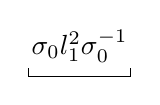
\begin{tikzpicture}[baseline=(term.base)]\node[inner sep=1pt] (term) {$\sigma_0l_1^2\sigma_0^{-1}$};\draw ([yshift=-1pt]term.south west) -- ++(0,-3pt) -| ([yshift=-1pt]term.south east);\end{tikzpicture}}\underset{\rho l_0}{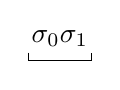
\begin{tikzpicture}[baseline=(term.base)]\node[inner sep=1pt] (term) {$\sigma_0\sigma_1$};\draw ([yshift=-1pt]term.south west) -- ++(0,-3pt) -| ([yshift=-1pt]term.south east);\end{tikzpicture}}l_\infty
=l_0l_\infty^2\rho l_0l_\infty
\]
thus finally
\[
(9)\quad\left\{\begin{aligned}
\varepsilon_0\varepsilon_1\deleted{\unsure{\varepsilon}}&=l_0l_\infty^2\rho l_0l_\infty\\
\varepsilon_1\varepsilon_\infty&=l_1l_0^2\rho l_1l_0\\
\varepsilon_\infty\varepsilon_0&=l_\infty l_1^2\rho l_\infty l_1
\end{aligned}\right.
\]
Eliminating the $l_i$ as $\varepsilon_i^2$, one finds generators $\varepsilon_0,\varepsilon_1,\varepsilon_\infty,\rho$, with \unsure{defining|defining} relations
\mspage{18}
